\documentclass[10pt,pdf,hyperref={unicode}]{beamer}

\mode<presentation>
{
\usetheme{boxes}
\beamertemplatenavigationsymbolsempty

\setbeamertemplate{footline}[page number]
\setbeamersize{text margin left=0.5em, text margin right=0.5em}
}

\usepackage[utf8]{inputenc}
\usepackage[english, russian]{babel}
\usepackage{bm}
\usepackage{multirow}
\usepackage{ragged2e}
\usepackage{indentfirst}
\usepackage{multicol}
\usepackage{subfig}
\usepackage{amsmath,amssymb}
\usepackage{enumerate}
\usepackage{mathtools}
\usepackage{comment}
\usepackage{multicol}

\usepackage[all]{xy}

\usepackage{tikz}
\usetikzlibrary{positioning,arrows}

\tikzstyle{name} = [parameters]
\definecolor{name}{rgb}{0.5,0.5,0.5}

\usepackage{caption}
\captionsetup{skip=0pt,belowskip=0pt}

\newtheorem{rustheorem}{Теорема}
\newtheorem{russtatement}{Утверждение}
\newtheorem{rusdefinition}{Определение}

% colors
\definecolor{darkgreen}{rgb}{0.0, 0.2, 0.13}
\definecolor{darkcyan}{rgb}{0.0, 0.55, 0.55}

\AtBeginEnvironment{figure}{\setcounter{subfigure}{0}}

\captionsetup[subfloat]{labelformat=empty}

%----------------------------------------------------------------------------------------------------------

\title[]{Adversarial training of Schrödinger bridges}
\author{Ksenofontov\,G.\,S.\\[1ex] 
\small Isachenko\,R.\,V.}
\institute[]{Moscow Institute of Physics and Technology}
\date[2023]{\small 20\;may\;2023}

%---------------------------------------------------------------------------------------------------------
\begin{document}

\begin{frame}
\titlepage
\end{frame}

%----------------------------------------------------------------------------------------------------------
\section{Research}
\begin{frame}{Research}
\bigskip
The problem of domain adaptation using  Schrödinger bridge problem is investigated.
\begin{block}{Research objective~---}
suggest a method of solving Schrödinger bridges using adversarial training.
\end{block}
\begin{block}{Required to suggest}
\justifying
\begin{enumerate}[1.]
    \item theory to connect adversarial training with Schrödinger bridges,
    \item algorithm of solving Schrödinger bridges using adversarial training.
\end{enumerate}
\end{block}
% \begin{block}{Solution}
% Для \ldots.
% \end{block}
\end{frame}
% %---------------------------------------------------------------------------------------------------------
\section{Problem statement}
\begin{frame}{Problem statement}
It is given
\begin{enumerate}[1.]
    \item $\{x_i\}_{i=0}^N, \{y_j\}_{j=0}^N \in \mathbb{R}^d$ -- two unpaired datasets,  where $x_i \sim \pi_0(x)$ and $y_j \sim \pi_1(y)$ ,
    \item $p^{\mathbb{W}^\gamma}= \mathcal{N}(0, \gamma\mathbb{I})$ -- conditional distribution, given by Wiener process with drift $\gamma$.
\end{enumerate}


\bigskip
We want to find joint distribution $p(x, y)$ that are constrained on $\pi_0(x)$ and $\pi_1(y)$. Static Schrödinger Bridge Problem find that distribution:
\begin{equation}
    \left\{ \begin{array}{c}
    p^*(x,y) = \arg\min_{p(x,y)} D_{KL}(p(x,y)||p^{\mathbb{W}^\gamma}(x,y)), \\
    \pi_0(x) = \int p(x,y)dy, \\
    \pi_1(y) = \int p(x,y)dx
    \end{array}\right.
    \label{eq:static}
\end{equation}

\end{frame}

% %----------------------------------------------------------------------------------------------------------
\section{Suggested Method}
\begin{frame}{Suggested Method}
~\\[-1mm]
To solve (\ref{eq:static}) is used Iterational Proportional fitting, which is alternates solving between two half bridges (constrained only on one distribution). However it can be mentioned that such algorithm could be rewritten as:
\begin{block}{Backward}
    \begin{equation*}
        \arg\min_{\phi, \psi} {\color{violet}D_{KL}(p_\phi(x)||\pi_0(x))} + {\color{blue}\mathbb{E}_{x\sim p_\phi(x)}\left[D_{KL}(p_\psi(y|x)||q^*_\omega(x|y))\right]} - \mathbb{E}_{x\sim p_\phi(x)}[\ln \pi_0(x)]
    \end{equation*}
\end{block}

\begin{block}{Forward}
    \begin{equation*}
        \arg\min_{\theta, \omega} {\color{violet}D_{KL}(q_\theta(x)||\pi_1(y))} + {\color{blue}\mathbb{E}_{y\sim q_\theta(y)}\left[D_{KL}(q_\omega(x|y)||p^*_\psi(y|x))\right]}  - \mathbb{E}_{y\sim q_\theta(y)}[\ln \pi_1(y)]
    \end{equation*}
\end{block}
\end{frame}
\begin{frame}{Suggested Method}
~\\[-1mm]
So, two marginal distributions could be learned with adversarial training and conditional distributions parameterised by normal distribution:
\begin{block}{Backward}
    \begin{equation*}
        \begin{split}
            \arg\min_{\phi, \psi}\max_{D_0} {\color{violet}\mathbb{E}_{x\sim \pi_0(x)}[D_0(x)] - \mathbb{E}_{x\sim p_\phi(x)}\left[e^{D_0(x) - 1}\right]} + \\
            + {\color{blue}\mathbb{E}_{x\sim p_\phi(x)}\left[D_{KL}(\mathcal{N}(y; \mu_\psi(x), \Sigma_\psi(x))||\mathcal{N}(x; \mu^*_\omega(y), \Sigma^*_\omega(y)))\right]} - \\ - \mathbb{E}_{x\sim p_\phi(x)}[\ln \pi_0(x)]
        \end{split}
    \end{equation*}
\end{block}

\begin{block}{Forward}
    \begin{equation*}
        \begin{split}
            \arg\min_{\theta, \omega}\max_{D_1} {\color{violet}\mathbb{E}_{y\sim \pi_1(y)}[D_1(y)] - \mathbb{E}_{y\sim q_\theta(y)}\left[e^{D_1(y) - 1}]\right]} + \\
            +  {\color{blue}\mathbb{E}_{y\sim q_\theta(y)}\left[D_{KL}(\mathcal{N}(x; \mu_\omega(y), \Sigma_\omega(y))||\mathcal{N}(y; \mu^*_\psi(x), \Sigma^*_\psi(x)))\right]} - \\ - \mathbb{E}_{y\sim q_\theta(y)}[\ln \pi_1(y)]
        \end{split}
    \end{equation*}
\end{block}
\end{frame}
\begin{frame}{Suggested Method}
~\\[-1mm]
    \begin{figure}
        \centering
        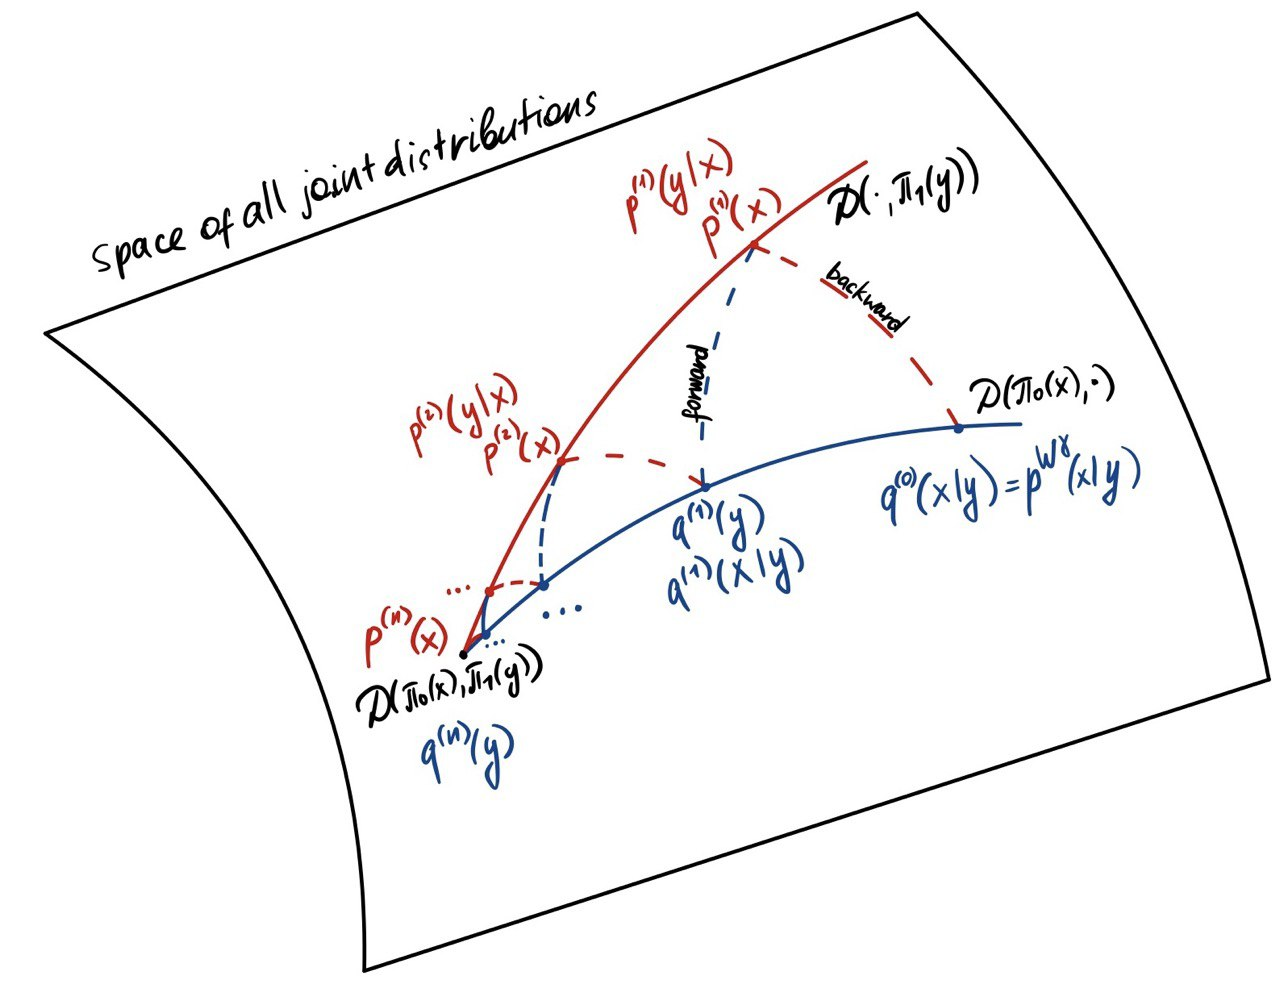
\includegraphics[width=0.8\linewidth]{slides/3d/figures/photo_2023-12-16_13-49-39.jpg}
    \end{figure}
\end{frame}
%---------------------------------------------------------------------------------------------------------
\section{Related papers}
\begin{frame}{Related papers}
\begin{enumerate}[1.]
    \item Machine-learning approaches for the empirical Schrodinger bridge problem\footnote{\href{https://www.cl.cam.ac.uk/techreports/UCAM-CL-TR-958.pdf}{Machine-learning approaches for the empirical Schrodinger bridge problem, F. Vargas, 2021}}
    \item f-GAN: Training Generative Neural Samplers using Variational Divergence Minimization\footnote{\href{https://arxiv.org/abs/1606.00709}{f-GAN: Training Generative Neural Samplers using Variational Divergence Minimization, S. Nowozin, 2016}}
\end{enumerate}
\end{frame}
%---------------------------------------------------------------------------------------------------------
\section{Additional information}
\begin{frame}{Additional information}
    Schrödinger Bridge Problem arises from Sanov's theorem, that allows us to measure probability of prior empirical stochastic process $\hat{\mathbb{W}}$ to be bounded between two given distributions $\pi_0(x)$ and $\pi_1(y)$:
    \begin{equation*}
        P\left(\hat{\mathbb{W}} \in \mathcal{D}(\pi_0, \pi_1)\right) \xrightarrow{N\rightarrow \infty} \exp\left(-N\inf_{\mathbb{P} \in \mathcal{D}(\pi_0, \pi_1)}D_{KL}\mathbb{(P||W})\right)
    \end{equation*}
    So the question arises: Is it possible to change somehow KL divergence to other distances or metrics?
\end{frame}
%---------------------------------------------------------------------------------------------------------
\section{Future work plan}
\begin{frame}{Future work plan}
\begin{enumerate}[1.]
    \item Make experiments with proposed adversarial training;
    \item Investigate generalization of $D_{KL}$ to other distances or metrics.
\end{enumerate}
\end{frame}

% %----------------------------------------------------------------------------------------------------------
% \section{Анализ предложенного метода \ldots}
% \begin{frame}{Анализ предложенного метода \ldots}
% \justifying

% На графике показана зависимость значения параметров$w_i$ в зависимости от параметра~$l_1$-регуляризации~$C$.
% \begin{figure}[h!]
% \includegraphics[width=0.45\textwidth]{../figures/log_reg_cs_exp.eps}
% \includegraphics[width=0.45\textwidth]{../figures/log_reg_cs_exp.eps}
% \end{figure}

% С увеличением параметра регуляризации~$C$ число ненулевых параметров~$w_i$ уменьшается.

% \end{frame}

% %----------------------------------------------------------------------------------------------------------
% \section{Выводы}
% \begin{frame}{Выводы}
% \justifying
% 	\begin{enumerate}
% 	\justifying
% 	    \item Предложен \ldots.
%         \item Доказаны теоремы \ldots, 
%         \begin{itemize}
%             \item[---] \ldots,
%             \item[---] \ldots.
%         \end{itemize}
%         \item Предложен метод \ldots
%         \begin{itemize}
%             \item[---] \ldots,
%             \item[---] \ldots.
%         \end{itemize}
%         \item Предложены методы \ldots
%         \begin{itemize}
%             \item[---] \ldots,
%             \item[---] \ldots.
%         \end{itemize}
%         \item Предложена вероятностная интерпретации \ldots.
% 	\end{enumerate}
% \end{frame}
% %----------------------------------------------------------------------------------------------------------

\end{document} 